\documentclass{article}

\usepackage{graphicx}
\usepackage{xepersian}

\settextfont{Vazirmatn}

\begin{document}

\begin{titlepage}

    % Center everything on the page
    \centering

    % Title
    \vspace*{2cm}
    {\Huge \textbf{تمرین دوم}} \\[1cm]
    
    % Subtitle
    {\LARGE درس مبانی برنامه نویسی و کامپیوتر} \\[2cm]
    
    % Author's name
    {\Large \textbf{دکتر ملکی مجد}} \\[0.5cm]
    
    % Date
    {\large \today} \\[4cm]
    
    % Semester
    {\large ترم پاییز ۴۰۳۱} \\[2cm]
    
    % Logo at the bottom
    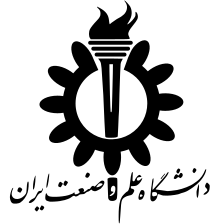
\includegraphics[width=0.2\textwidth]{iustlogo.png} \\[0.2cm]
    \textbf{دانشگاه علم و صنعت}
    
\end{titlepage}

\section{نکات}
\begin{enumerate}
    \item  پاﺳﺦ ﺗﻤﺎمی ﺳﻮاﻻت ﺗﻨﻬﺎ ﺑﺎ زﺑﺎن ﺳی ﻗﺎﺑﻞ ﻗﺒﻮل اﺳﺖ.
    \item در صورتی که در هر سؤال ابهام یا سوالی وجود داشت. حتما سعی کنید سؤال خود را
    در گروه درسی بپرسید تا دیگران نیز از پاسخ شما بهره‌مند شوند.
    \item در صورتی که از منابعی برای حل سوالات استفاده کرده اید حتما آن را به صورت کامنت
    در ابتدای کدخود بنویسید. همچنین اگر با دانشجو دیگری همفکری کرده اید حتما آن
    را نیز ذکر کنید.
    \item برای ارسال تمرین های خود در طول ترم مجموعا ۱۰ روز تاخیر مجاز وجود دارد. در
    صورتی که بیشتر از این مقدار تاخیر داشته باشید، نمره تمرین شما صفر خواهد شد.
    \item برای هر سری تمرین ۳ روز از ۱۰ روز تاخیر مجاز را می توانید استفاده کنید.
\end{enumerate}

\section{طراحان سؤال}
در صورتی که در هر سوالی ابهامی وجود دارد، میتونید از طریق آیدی های زیر سؤال خود را
مطرح کنید.

\begin{itemize}
    \item عرفان ابراهیمی - \lr{ID: @erfebs}
    \item آرین عبدالهی ثابت نژاد - \lr{ID: @aryan\_sabet}
\end{itemize}

\pagebreak

\section{معدل‌گیری نمرات دانشجویان}

علی، که تازه وارد دانشگاه شده، تصمیم گرفته برنامه‌ای بنویسد تا نمرات دروس خود و دوستانش را تحلیل کند. او می‌خواهد میانگین نمرات، بالاترین نمره، و پایین‌ترین نمره را محاسبه کند. به او کمک کنید تا این برنامه را بنویسد. اما استادی به او گیر داده است که باید میانگین نمرات چند کلاس او را هم محاسبه کند. به علی کمک کنید تا این مسئله را حل کند.

\subsection{ورودی}

در خط اول تعداد کلاس هایی که نمرات آن ها قرار است محاسبه شود آمده است. در هر کلاس، ابتدا
تعداد دانشجویان کلاس و سپس نمرات آن‌ها به صورت اعداد صحیح مثبت آمده است. تعداد دانشجویان هر کلاس حداکثر 100 نفر است و نمرات هر دانشجو حداکثر 20 است.

\subsection{خروجی}

بعد از ورود اطلاعات هر کلاس بایستی شماره کلاس و میانگین نمرات، بالاترین نمره و پایین‌ترین نمره آن کلاس چاپ شود. میانگین نمرات باید تا دو رقم اعشار چاپ شود.
در آخر هم شماره کلاس با کمترین و بیشترین میانگین نمرات چاپ شود. اگر چند کلاس میانگین
یکسان داشتند، کلاس با بیشترین شماره چاپ شود.

\subsection{مثال‌ها}

\paragraph{نمونه ۱:}

\textbf{ورودی:}
\begin{LTR}
\begin{verbatim}
5
3
14 15 20
4
10 12 14 16
2
10 20
3
14 15 16
4
10 12 14 16
\end{verbatim}
\end{LTR}

\textbf{خروجی:}
\begin{LTR}
\begin{verbatim}
Class 1:
Average: 16.33
Max: 20
Min: 14
Class 2:
Average: 13.00
Max: 16
Min: 10
Class 3:
Average: 15.00
Max: 20
Min: 10
Class 4:
Average: 15.00
Max: 16
Min: 14
Class 5:
Average: 13.00
Max: 16
Min: 10
Class with highest average: 1
Class with lowest average: 5
\end{verbatim}
\end{LTR}

\paragraph{نمونه ۲:}

\textbf{ورودی:}
\begin{LTR}
\begin{verbatim}
2
3
10 10 10
3
20 20 20
\end{verbatim}
\end{LTR}

\textbf{خروجی:}
\begin{LTR}
\begin{verbatim}
Class 1:
Average: 10.00
Max: 10
Min: 10
Class 2:
Average: 20.00
Max: 20
Min: 20
Class with highest average: 2
Class with lowest average: 1
\end{verbatim}
\end{LTR}

\newpage

\section{جمع ارقام}

علی تازه با برنامه‌نویسی آشنا شده است. برای تمرین، می‌خواهد برنامه‌ای بنویسد که جمع ارقام یک عدد را محاسبه کند. به او کمک کنید تا این مسئله را حل کند.

\subsection{ورودی}

ورودی شامل یک خط است که در آن یک عدد صحیح \( n \) آمده است.

\subsection{خروجی}

در خروجی باید جمع ارقام عدد \( n \) را چاپ کنید.

\subsection{مثال‌ها}

\paragraph{نمونه ۱:}

\textbf{ورودی:}
\begin{LTR}
\begin{verbatim}
123
\end{verbatim}
\end{LTR}

\textbf{خروجی:}
\begin{LTR}
\begin{verbatim}
6
\end{verbatim}
\end{LTR}

\paragraph{نمونه ۲:}

\textbf{ورودی:}
\begin{LTR}
\begin{verbatim}
5040
\end{verbatim}
\end{LTR}

\textbf{خروجی:}
\begin{LTR}
\begin{verbatim}
9
\end{verbatim}
\end{LTR}

\paragraph{نمونه ۳:}

\textbf{ورودی:}
\begin{LTR}
\begin{verbatim}
0
\end{verbatim}
\end{LTR}

\textbf{خروجی:}
\begin{LTR}
\begin{verbatim}
0
\end{verbatim}
\end{LTR}

\newpage

\section{لوزی}

علی در حال یادگیری برنامه‌نویسی است و تصمیم گرفته است با استفاده از حلقه‌ها یک الگوی لوزی شکل بسازد. شما باید به او کمک کنید تا این مسئله را حل کند.

\subsection{ورودی}

ورودی شامل یک عدد صحیح \( n \) است که بیانگر نصف ارتفاع الگوی لوزی به علاوه یک است.

\subsection{خروجی}

باید الگوی لوزی مطابق مقدار \( n \) را چاپ کنید.

\subsection{مثال‌ها}

\paragraph{نمونه ۱:}

\textbf{ورودی:}
\begin{LTR}
\begin{verbatim}
5
\end{verbatim}
\end{LTR}

\textbf{خروجی:}
\begin{LTR}
\begin{verbatim}
    *
   ***
  *****
 *******
*********
 *******
  *****
   ***
    *
\end{verbatim}
\end{LTR}

\paragraph{نمونه ۲:}

\textbf{ورودی:}
\begin{LTR}
\begin{verbatim}
3
\end{verbatim}
\end{LTR}

\textbf{خروجی:}
\begin{LTR}
\begin{verbatim}
  *
 ***
*****
 ***
  *
\end{verbatim}
\end{LTR}

\newpage

\section{اعداد اول}

علی در حال یادگیری اعداد اول است. او می‌خواهد برنامه‌ای بنویسد که تمامی اعداد اول کوچکتر یا مساوی یک عدد مشخص را پیدا کند. به او کمک کنید تا این مسئله را حل کند.

\subsection{ورودی}

در تنها خط ورودی یک عدد صحیح مثبت \( n \) (بزرگ‌تر یا مساوی 2) داده می‌شود.

\subsection{خروجی}

تمامی اعداد اول کوچکتر یا مساوی \( n \) در یک خط چاپ شوند و با فاصله از یکدیگر جدا شوند.

\subsection{مثال‌ها}

\paragraph{نمونه ۱:}

\textbf{ورودی:}
\begin{LTR}
\begin{verbatim}
10
\end{verbatim}
\end{LTR}

\textbf{خروجی:}
\begin{LTR}
\begin{verbatim}
2 3 5 7
\end{verbatim}
\end{LTR}

\paragraph{نمونه ۲:}

\textbf{ورودی:}
\begin{LTR}
\begin{verbatim}
20
\end{verbatim}
\end{LTR}

\textbf{خروجی:}
\begin{LTR}
\begin{verbatim}
2 3 5 7 11 13 17 19
\end{verbatim}
\end{LTR}

\paragraph{نمونه ۳:}

\textbf{ورودی:}
\begin{LTR}
\begin{verbatim}
2
\end{verbatim}
\end{LTR}

\textbf{خروجی:}
\begin{LTR}
\begin{verbatim}
2
\end{verbatim}
\end{LTR}

\newpage

\section{دنباله فیبوناچی}

علی در حال یادگیری دنباله فیبوناچی است. او می‌خواهد برنامه‌ای بنویسد که دنباله فیبوناچی را تا جمله‌ی \( n \)ام محاسبه کند. به او کمک کنید تا این برنامه را پیاده‌سازی کند.

\subsection{تعریف دنباله فیبوناچی}

\begin{itemize}
    \item جمله اول و دوم دنباله برابر با 0 و 1 هستند.
    \item هر جمله بعدی برابر است با مجموع دو جمله قبل از آن. 
\end{itemize}

\subsection{ورودی}

در تنها خط ورودی یک عدد صحیح مثبت \( n \) (بزرگ‌تر یا مساوی 1) داده می‌شود که نشان‌دهنده تعداد جملات موردنظر از دنباله است.

\subsection{خروجی}

در خروجی باید \( n \) جمله اول دنباله فیبوناچی چاپ شود. جملات با فاصله از یکدیگر جدا شوند.

\subsection{مثال‌ها}

\paragraph{نمونه ۱:}

\textbf{ورودی:}
\begin{LTR}
\begin{verbatim}
5
\end{verbatim}
\end{LTR}

\textbf{خروجی:}
\begin{LTR}
\begin{verbatim}
0 1 1 2 3
\end{verbatim}
\end{LTR}

\paragraph{نمونه ۲:}

\textbf{ورودی:}
\begin{LTR}
\begin{verbatim}
10
\end{verbatim}
\end{LTR}

\textbf{خروجی:}
\begin{LTR}
\begin{verbatim}
0 1 1 2 3 5 8 13 21 34
\end{verbatim}
\end{LTR}

\paragraph{نمونه ۳:}

\textbf{ورودی:}
\begin{LTR}
\begin{verbatim}
1
\end{verbatim}
\end{LTR}

\textbf{خروجی:}
\begin{LTR}
\begin{verbatim}
0
\end{verbatim}
\end{LTR}

\end{document}

